\documentclass{article}

\usepackage{../arxiv}

\usepackage[utf8]{inputenc} % allow utf-8 input
\usepackage[T1]{fontenc}    % use 8-bit T1 fonts
\usepackage{hyperref}       % hyperlinks
\usepackage{url}            % simple URL typesetting
\usepackage{booktabs}       % professional-quality tables
\usepackage{amsfonts}       % blackboard math symbols
\usepackage{nicefrac}       % compact symbols for 1/2, etc.
\usepackage{microtype}      % microtypography
\usepackage{cleveref}       % smart cross-referencing
\usepackage{graphicx}
\usepackage{caption}
\usepackage{algorithm}
\usepackage{algpseudocode}
\usepackage{ragged2e}
\usepackage[style=numeric,sorting=none]{biblatex}
\usepackage[symbol]{footmisc}
\usepackage{tabu}
\usepackage{color}
\usepackage{nicefrac}

\addbibresource{\jobname.bib}

\title{Dango DEX}

\author{
  Larry Engineer \\
	Left Curve Software \\
	\texttt{larry@leftcurve.io} \\
}

\date{Initial version: UNRELEASED}

\begin{document}
\maketitle

\begin{abstract}
  Dango is an onchain limit order book exchange that tackles three main challenges faced by today's decentralized exchanges: 1) inaccessibility of order book market making to retail investors due to the high level of sophistication required; 2) value leak from passive liquidity pools due to arbitrage flow; 3) sandwich attacks. Dango enshrines its order book with a passive liquidity pool that actively adjusts its quotes utilizing a low latency oracle, and clears orders using frequent, uniform price, sealed bid auctions. Overall, Dango seeks to democratize market making on order books, minimize toxic arbitrage flow, while maximize organic, non-arbitrage flow.
\end{abstract}

\section{Background}

\subsection{TradFi}

In traditional finance (TradFi) markets, \textbf{limit order book} (LOB) is the primary venue for trading. A limit order consists of the quantity of asset the trader wishes to buy or sell, and a limit price at which or better the trade must be executed.

\textbf{Market makers} (MMs) facilitate trades by strategically placing orders below and above the prevailing market price. E.g., suppose Apple stock (AAPL) is trading at \$200. An MM may place a \texttt{BUY} order at \$199.5 and a \texttt{SELL} order at \$200.5. The \$1 difference is known as the \textbf{spread}. If a trader sells one share of AAPL to the MM at \$199.5, then another trader buys the share at \$200.5, the MM has made \$1. This is typically described as the MM ``making money on the spread''.

MMs bet the stock's price goes side ways, i.e. there is roughly the same buy and sell volume. If the market only goes one way, the MM accumulates one side of the inventory, which is the underperforming side. E.g., if there is consistently more sellers of AAPL than buyers, the MM's \texttt{BUY} orders get consistently picked up more often than his \texttt{SELL} orders do, he would accumuate a large inventory of AAPL, an asset that's going down in price. He would underperform the trading strategy of simply holding the initial inventory and doing nothing. This is known as the \textbf{inventory risk} which is rooted in the asset's price volatility. MMs usually use \textbf{hedging} to mitigate this risk.

Another major risk faced by MMs comes from \textbf{frontrunning}. Suppose Apple releases a better-than-expected earnings report, causing the ``fair value'' of its stock to jump to \$300. However, the MM is still placing orders around the \textbf{stale price} of \$200, either because he isn't aware of the news or is slow to update the quotes. A \textbf{high frequency trader} (HFT) is one who is well informed on the news and is able to execute trades faster. The HFT is able to pick up the MM's \texttt{SELL} order at \$200.5 and immediately resell the stock for \$300, pocketing the arbitrage gain. The MM loses value because he has sold the stock at a much lower-than-market price. Both MMs and HFTs invest significant amount of resources to improve their execution speed in an ``arms race''.\supercite{frequentbatchauctions} This is a very high level of sophistication that makes market making on LOBs inaccessible to most retail investors.

\subsection{DeFi}

Maintaining a LOB and executing orders is computationally costly. For this reason, onchain finance has historically relied on \textbf{constant function market makers} (CFMMs) instead of LOBs. (That is, until the recent advent of high performance blockchains such as Solana, Diem, and Hyperliquid.)

A CFMM, instead of maintaining a book of limit orders, maintains a pool of liquidity and quotes prices based on a predefined \textbf{invariant}. An invariant is a function $f(x, y)$ that yields the same value before and after a trade, where $x$ and $y$ are the quantities of the \textbf{base asset} and the \textbf{quote asset}, respectively (known as the pool's \textbf{reserves}):

\begin{equation}
  f(x, y) = \mathrm{constant}
\end{equation}

Suppose a pool contains base asset $\mathtt{A}$ and quote asset $\mathtt{B}$ of reserves $A$ and $B$, respectively, and a trader wishes to swap $a$ units of $\mathtt{A}$ into $\mathtt{B}$. The pool would determine the output amount $b$ by solving the equation:

\begin{equation}
  f(A, B) = f(A + a, B - b)
\end{equation}

Similarly, a swap from $b$ units of $\mathtt{B}$ into $\mathtt{A}$ will have its output amount $a$ determined by:

\begin{equation}
  f(A, B) = f(A - a, B + b)
\end{equation}

Note that this doesn't consider trading fees. Since there is no such thing as ``spread'' in CFMMs as in LOBs, the pool makes money for its \textbf{liquidity providers} (LPs) by charging a fee on each trade. Specifically, a small portion of the trade's output is deducted and injected into the pool. The value of $f(x, y)$ slightly increases as a result. As such, $f(x, y)$ can be considered as a measurement of how much liquidity there is in the pool, regardless of the asset prices.

CFMMs share the same types of risks as LOBs, but to different degrees. Firstly, LPs in an CFMM pool bet the two assets' relative price stays roughly constant. If one asset's price drops relative to the other, the pool accumulates this underperforming asset. Not considering fees, this would underperform the strategy of simply holding the two assets and doing nothing. This is commonly called \textbf{impermanent loss} (IL), an arguably bad naming as the loss isn't guaranteed to be ``impermanent''. IL is essentially the same thing as inventory risk for LOBs, caused by the asset's volatility, and can be mitigated by hedging.

In terms of frontrunning, however,  CFMMs are categorically worse than LOBs. A traditional CFMM \textit{never} adjusts its quotes in response to new information. Therefore, from an LP's perspective, a CFMM \textit{always} trades at worse-than-market prices. HFTs can siphone values from the liquidity pool by executing CEX-DEX arbitrage, similarly as described in the previous section. The loss that LPs suffer due to arbitrage activities can be quantified as \textbf{loss-versus-rebalancing} (LVR).\supercite{lvr}

Traders on DEXs are susceptible to \textbf{sandwich attacks}, where an attacker inserts transactions immediately before and after a trade. These transactions manipulate prices in the DEX, give the trader a worse execution price, while profiting the attacker. Sandwich attack is not inheritly a problem of CFMMs; onchain LOBs can be similarly attacked. Fundamentally, it's a result of user orders being broadcasted transparently through a public network. In contrast, TradFi traders broadcast directly to the exchanges through private channels.

Both arbitrage and sandwich attack require transactions in blocks to be ordered in specific ways. To achieve this, actors executing these trades bribe the block builders via revenue share. The aggregate amount of revenue shared with block builders is known as \textbf{miner extractable value} (MEV), as in proof-of-work blockchains it's the miners who play the role of block builders.

\subsection{The problems}

Through the above discussions, we have identified three problems with today's decentralized exchanges (DEXs):

\begin{enumerate}
  \item Market making in LOBs is not accessible to retail investors because of the high level of sophistication required, which is in larger part a result of the HFT arms race.
  \item CFMM democratizes market making to retail investors, but they generally don't make money or even lose money because of LVR.
  \item Traders are susceptible to sandwich attacks due to the lack of privacy.
\end{enumerate}

We do not aim to solve IL, because it's rooted in the assets' volalitity, not a problem with DEX design. We can imagine automated vaults that mitigate it by deploying hedging strategies.

\section{Our solution}

We propose solving the above problems as follows:

\begin{itemize}
  \item Create a LOB that has an enshrined passive liquidity pool. The pool will place orders in the LOB following a CFMM invariant.
  \item In order to mitigate LVR, we:
        \begin{itemize}
          \item make available a high-frequency, low-latency oracle reporting the latest prevailing market prices;
          \item incorporate this oracle feed into the liquidity pool's CFMM invariant;
          \item give the pool priority in adjusting its quotes over other traders.
        \end{itemize}
  \item In order to mitigate MEV, we:
        \begin{itemize}
          \item use a private mempool so that user orders aren't public;
          \item execute orders frequent, uniform price, sealed bid auctions, so that HFTs don't have time advantage over other traders.
        \end{itemize}
\end{itemize}

The rest of this paper discusses these points in detail. First, let's discuss how to incorporate a passive CFMM pool into a LOB.

\subsection{Passive liquidity on a LOB}

First, we introduce the concept of \textbf{marginal price}, $p_{\mathrm{m}}$, of a CFMM. This is the price (defined as the units of quote asset that is equivalent in value as one unit of base asset) a trader gets if swapping an infinitesimal amount of base asset into the quote asset. Given an invariant $f(x, y)$, it can be evaluated as:

\begin{equation}
  p_{\mathrm{m}} = - \frac{\mathrm{d}y}{\mathrm{d}x} = \frac{\frac{\partial f}{\partial x}}{\frac{\partial f}{\partial y}}
\end{equation}

Our passive liquidity pool will place \texttt{BUY} orders at prices below $p_{\mathrm{m}}$, \texttt{SELL} orders above $p_{\mathrm{m}}$, and no order at exactly $p_{\mathrm{m}}$.

Let us consider the \texttt{BUY} side first. Suppose the pool has reserves $A$ units of base asset and $B$ units of quote asset. Consider a swap that inputs $a$ units of base asset and outputs $b$ units of quote asset. The swap must follow the invariant:

\begin{equation}
  f(A, B) = f(A + a, B - b)
\end{equation}

We say the execution price of this trade is $p = \frac{b}{a}$.

We intrepret this as follows: the pool is willing to buy $a$ units of the base asset from counterparty traders at price $p$. In the context of LOB, this means the pool would put a cumulative \texttt{BUY} demand of quantity $a$ from $p_{\mathrm{m}}$ to $p$.

In reality, price is not continuous; the pool can only put orders at discrete \textbf{ticks}. Denote \textbf{tick size} as $\Delta p$, and the $n$-th tick below $p_{\mathrm{m}}$ as $p_n$:

\begin{equation}
  p_n = p_{\mathrm{m}} - n \Delta p \ \ (n = 0, 1, 2, \dots)
\end{equation}

If we find the pool places a cumulative \texttt{BUY} demand of quantity $a_n$ at price $p_n$, and quantity $a_{n-1}$ at price $p_{n-1}$, then obviously the order to be put at price $p_n$ is:

\begin{equation}
  \Delta a_n = a_n - a_{n-1}
\end{equation}

With $a_0 = 0$, we can iteratively work out $\Delta a_n$ for all $n = 1, 2, 3, \dots$; see \hyperref[alg:1]{Algorithm 1}.

\begin{algorithm}
  \caption{Determine \texttt{BUY} order sizes at ticks $p_n$, $n = 1, 2, 3, \dots$}
  \label{alg:1}
  \begin{algorithmic}
    \State $p_0 \gets p_{\mathrm{m}}$
    \State $a_0 \gets 0$
    \State $\Delta a_0 \gets 0$
    \For{n = 1, 2, 3, \dots}
    \State $p_n \gets p_{n-1} - \Delta t$
    \State $a_n \gets a: f(A, B) = f(A + a, b - p_n a)$ \Comment{Solve the invariant equation}
    \State $\Delta a_n \gets a_n - a_{n-1}$
    \EndFor
    \State \Return $[p_1, p_2, \dots]$, $[a_1, a_2, \dots]$, $[\Delta a_1, \Delta a_2, \dots]$
  \end{algorithmic}
\end{algorithm}

For the \texttt{SELL} side, the procedure is similar; \hyperref[alg:2]{Algorithm 2}.

\begin{algorithm}
  \caption{Determine \texttt{SELL} order sizes at ticks $p_n$, $n = 1, 2, 3, \dots$}
  \label{alg:2}
  \begin{algorithmic}
    \State $p_0 \gets p_{\mathrm{m}}$
    \State $a_0 \gets 0$
    \State $\Delta a_0 \gets 0$
    \For{n = 1, 2, 3, \dots}
    \State $p_n \gets p_{n-1} + \Delta t$
    \State $a_n \gets a: f(A, B) = f(A - a, b + p_n a)$ \Comment{Solve the invariant equation}
    \State $\Delta a_n \gets a_n + a_{n-1}$
    \EndFor
    \State \Return $[p_1, p_2, \dots]$, $[a_1, a_2, \dots]$, $[\Delta a_1, \Delta a_2, \dots]$
  \end{algorithmic}
\end{algorithm}

\subsection{Xyk}

The simplest yet the widely used CFMM invariant is the \textbf{xyk invariant},\supercite{xykamm} which has the form:

\begin{equation}
  f(x, y) = xy
\end{equation}

Marginal price can be found as:

\begin{equation}
  p_{\mathrm{m}} (x, y) = \frac{y}{x}
\end{equation}

It's easy to solve that for the \texttt{BUY} side:

\begin{equation}
  a = -A + \frac{B}{p}
\end{equation}

For the \texttt{SELL} side:

\begin{equation}
  a = A - \frac{B}{p}
\end{equation}

\textbf{Example.} Consider a pool containing base asset SOL of quantity $A = 1$ and quote asset USD of quantity $B = 200$. marginal price $p_{\mathrm{m}} = 200$. Following \hyperref[alg:1]{Algorithms 1} and \hyperref[alg:2]{2} we can work out the order sizes in relation to tick price ($\Delta a_n$--$p_n$) and cumulative order depth ($a_n$--$p_n$), plotted in \hyperref[fig:1]{Figure 1}.

\begin{figure}
  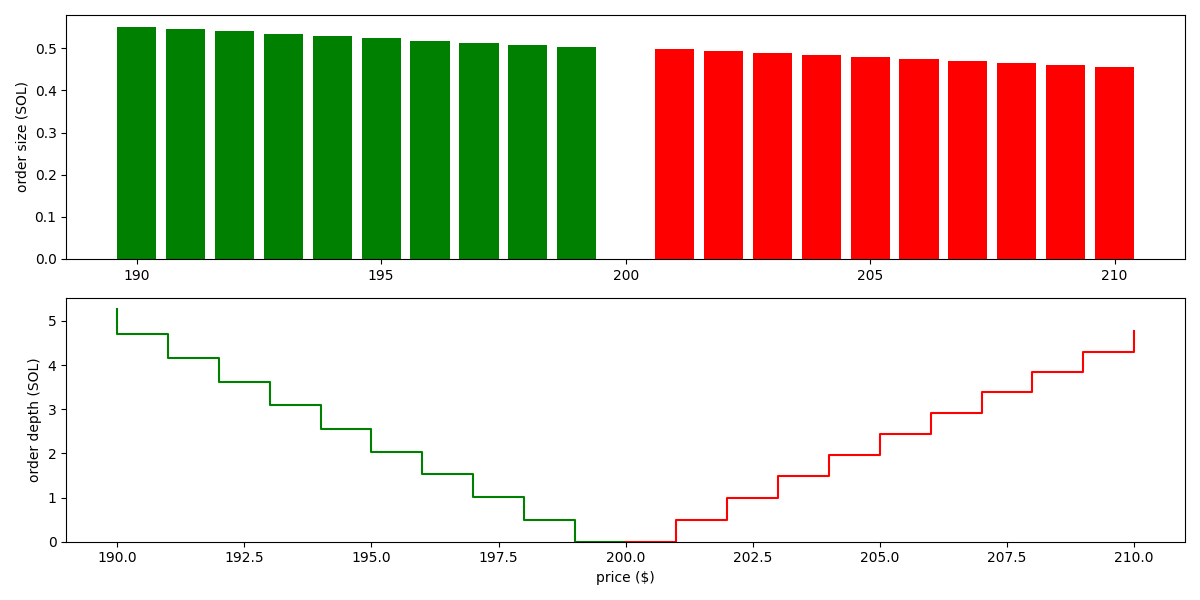
\includegraphics[width=\textwidth]{1-xyk.png}
  \caption{Order size and depth following the xyk invariant. $A = 1$, $B = 200$, $\Delta p = 0.1$.}
  \label{fig:1}
\end{figure}

We can see the pool puts liquidity roughly evenly over a wide range of prices. This is capital inefficient; ideally, we want to concentrate the liquidity in the region close to $p_{\mathrm{m}}$.

Additionally, this invariant is susceptible to LVR, as $p_{\mathrm{m}}$ does not adjust in response to the change of price in CEXs.

\subsection{Solidly}

The Solidly invariant, conceived by Andre Cronje,\supercite{andrecronjetwitter} has the form:

\begin{equation}
  f(x, y) = x^3 y + x y^3 = K
\end{equation}

This formula assumes the two assets have the same price. In case they're not the same price, and we have an oracle feed indicating that one unit of $x$ is equivalent in value to $R$ units of $y$, the formula can be modified to:

\begin{equation}
  f(x, y) = x^3 \left( \frac{y}{R} \right) + x \left( \frac{y}{R} \right)^3
\end{equation}

The marginal price is:

\begin{equation}
  p_{\mathrm{m}} (x, y) = \frac{3 R^2 x^2 y + y^3}{R^2 x^3 + 3 x y^2}
\end{equation}

For convenience, let's denote:

\begin{equation}
  \alpha = A + a
\end{equation}

\begin{equation}
  \beta = \frac{B - p a}{R}
\end{equation}

Essentially, $\alpha$ is the pool's base asset reserve after the trade, $\beta$ is the quote asset reserve after the trade, adjusted for the oracle price.

The invariant equation:

\begin{equation}
  f(A, B) = f(A + a, B - p a) = \alpha^3 \beta + \alpha \beta^3
\end{equation}

This is a 4th-degree (quartic) equation, so finding a closed form solution is not feasible. Instead, we solve it using \textbf{Newton's method}. Define:

\begin{equation}
  g(a) = \alpha^3 \beta + \alpha \beta^3 - f(A, B)
\end{equation}

\begin{equation}
  g'(a) = -\frac{p}{R} \alpha^3 + a \alpha^2 \beta - \frac{3p}{R} \alpha \beta^2 + \beta^3
\end{equation}

We solve for $a$ such that $g(a) = 0$ following \hyperref[alg:3]{Algorithm 3}.

\begin{algorithm}
  \caption{Newton's method for solving $g(a) = 0$}
  \label{alg:3}
  \begin{algorithmic}
    \State $a_0 \gets A$
    \For{$i = 1, 2, 3, \dots$}
    \State $a_i \gets a_{i-1} - \frac{g(a_{i-1})}{g'(a_{i-1})}$
    \If{converge}
    \State \Return $a_i$ as the solution
    \EndIf
    \EndFor
  \end{algorithmic}
\end{algorithm}

The choice of the initial value $a_0$ is important. This is because $g(a) = 0$ has a trivial solution of $a = 0$, which corresponding to not placing an order at all. Instead, we want to find the non-trivial solution of $a > 0$. Emprically, choosing $a_0 = A$ always gives us the intended solution.

For the \texttt{SELL} side:

\begin{equation}
  \alpha = A - a
\end{equation}

\begin{equation}
  \beta = \frac{B + p a}{R}
\end{equation}

\begin{equation}
  g(a) = \alpha^3 \beta + \alpha \beta^3 - f(A, B)
\end{equation}

\begin{equation}
  g'(a) = \frac{p}{R} \alpha^3 - a \alpha^2 \beta + \frac{3p}{R} \alpha \beta^2 - \beta^3
\end{equation}

\textbf{Example.} Following the same example of SOL-USD pool in the previous discussions, assuming oracle price $R = 200$ (USD per SOL), the liquidity depth can be computed and plotted in \hyperref[fig:2]{Figure 2}. It's obvious that liquidity is now indeed concentrated around the marginal price.

\begin{figure}
  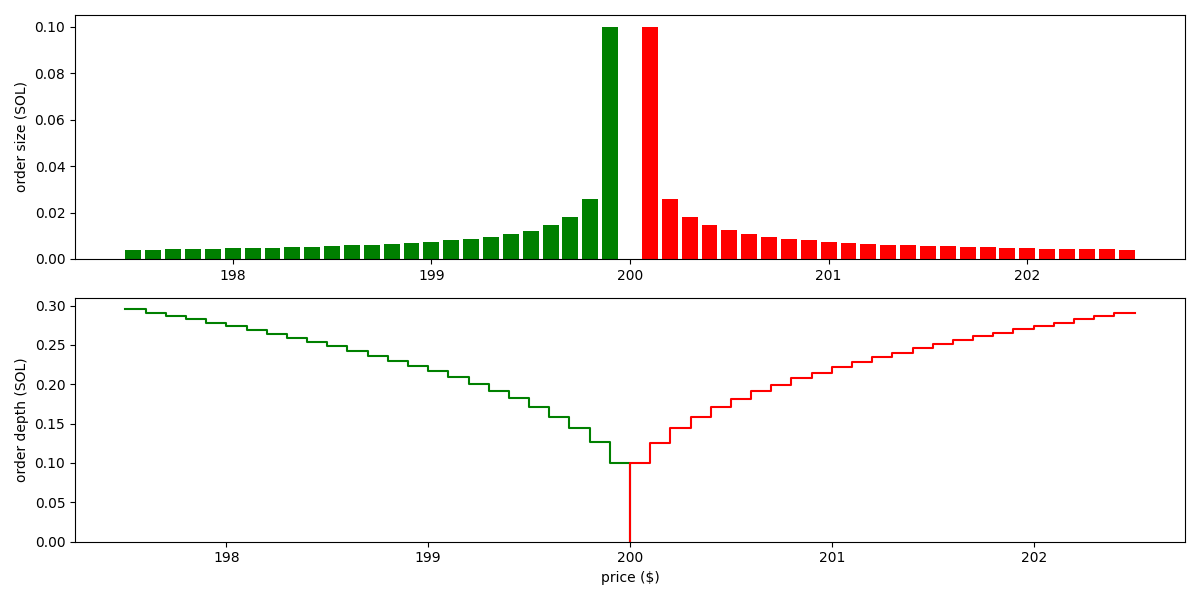
\includegraphics[width=\textwidth]{2-solidly.png}
  \caption{Order size and depth following the Solidly invariant. $A = 1$, $B = 200$, $\Delta p = 0.1$, $R = 200$.}
  \label{fig:2}
\end{figure}

In general, however, $R$ and $p_{\mathrm{m}}$ do not match exactly. In TradFi, MMs typically respond to this by adjusting the spread.\supercite{avellanedastoikov} Consider the situation where SOL appreciates to $R = 210$. In this case, a TradFi MM would \textit{increase} the bid spread and \textit{decrease} the ask spread. Thus, there is a higher probability the asks are picked up by traders, such that the MM offloads SOL and intakes USD, trending towards a rougly 1:1 ratio in value of the two assets.

How will our passive liquidity pool respond to this situation? Let's plot it in \hyperref[fig:3]{Figure 3}. As we see, the pool keeps the same spread on each side, but less \texttt{BUY} demand and more \texttt{SELL} demand. This indicates the pool has a similar tendency of offloading SOL and intaking USD in this situation.

\begin{figure}
  \centering
  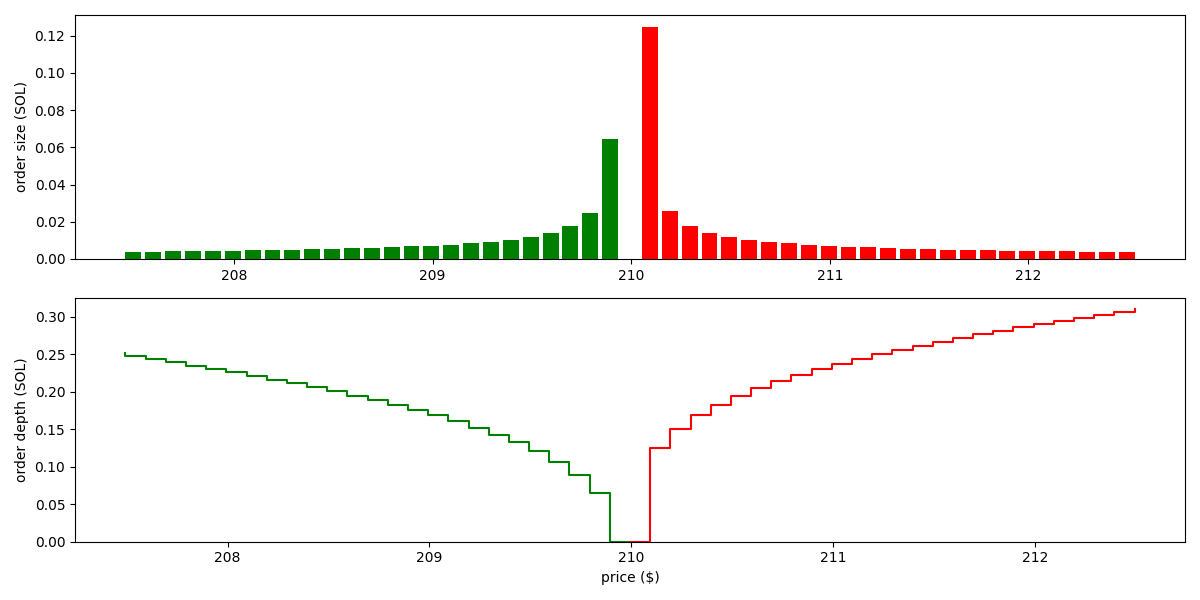
\includegraphics[width=\textwidth]{3-solidly-price-jump.png}
  \caption{Order size and depth following the Solidly invariant. $A = 1$, $B = 200$, $\Delta p = 0.1$, $R = 210$.}
  \label{fig:3}
\end{figure}

\subsection{Minimizing LVR with oracle-imformed CFMM}

In order for the passive liquidity pool to provide accurate quotes and not leak value to arbitrageurs, it's important that:

\begin{itemize}
  \item it has access a low-latency oracle which provides the price $R$; and,
  \item it must be able to adjust its orders before any other trader is able to pick up the stale quotes.
\end{itemize}

We propose using Pyth Laser\supercite{pythlaser} as the data source for $R$, which provides ultra fast price feeds with 1 millisecond updates.

\textbf{On oracle risk.} A concern over oracle-informed CFMMs is that an inaccurate oracle price can cause unbounded loss for LPs.\supercite{riskoforacleamm} We propose two ways to safeguard against this:

\begin{itemize}
  \item Pyth's price feed comes with a \textbf{confidence interval}.\supercite{pythconfidenceinterval} We propose the passive liquidity pool to always place orders outside this interval. For example, suppose Pyth reports the price of SOL is $\$200 \pm 0.5$. In this case, the pool will place bids below $200 - 0.5 = 199.5$, and asks above $200 + 0.5 = 200.5$. Generally, the interval is less than 0.1\%, so the pool's quotes are still attractive for traders.
  \item The pool should ensure the oracle price isn't too old, by checking its age against a preset threshold. If too old, the pool will not place any order in the book, until a sufficiently new feed is received.
\end{itemize}

\subsection{Mitigating MEV with frequent batch auctions}

A sandwich attacker relies on two prerequisites both being satisfied in order to pull off an attack:

\begin{itemize}
  \item user orders are broadcasted transparently, unencrypted, through a public network;
  \item trades are possibly executed at different prices throughout the same block.
\end{itemize}

On the first point, we believe the endgame solution is implementing an encrypted mempool.\supercite{encryptedmempool} However, to achieve a faster go-to-market, we propose an interim solution: 1) the Dango chain to temporarily run on a proof-of-authority validator set; 2) validators to configure their mempools such that they only receive transactions, and broadcast only to other validators, but not to any non-validator node; 3) users to broadcast their transactions directly to the validators. As such, user transactions can be considered effectively private, as no one other than the validators has access to them.

On the second point, we propose to execute orders using frequent batch auctions (FBAs).\supercite{frequentbatchauctions} FBAs operate as follows: during a preset time interval, typically 0.2--1.0 second, the exchange accepts orders from traders. It does not execute these order yet; instead, stores them in a private book separate from the main book. At the end of the interval, the exchange combines orders in the two books, and performs a uniform price auction to find a single clearing price. Specifically, this price is the intersection between the cumulative supply and demand curves. At this price, trading volume (measured in units of the base asset) is maximized. As all orders are settled at the same price, it's impossible to execute sandwich attacks.

\subsection{Implementation}

Putting together the points proposed above, we suggest the following implementation.

First, the Dango chain will utilize a centralized block builder who, when building a block, will first fetch the latest oracle data from Pyth's API, and insert a transaction to the top of block that submits the data onchain. The data is to be signed by a trusted party, typically the Wormhole guardian set,\supercite{wormholeguardianset} and verified onchain.

The follow of the block is as follows:

\begin{enumerate}
  \item The first transaction is always the oracle update.
  \item For each of the other transactions:
        \begin{itemize}
          \item If it's to cancel an order, immediately perform the cancellation.
          \item If it's to place an order, insert the order into the private book.
        \end{itemize}
  \item Once all transactions have been processed, perform order clearing:
        \begin{enumerate}
          \item First, compute the orders to be placed by the passive liquidity pool, given the latest oracle price $R$. It's important this is done first, so that the pool doesn't leave any stale quotes.
          \item Merge the private book into the main book.
          \item Iterate through orders in the main book and those placed by pool together, and find the clearing price.
          \item Fill the orders at this price.
        \end{enumerate}
\end{enumerate}

\section{Conclusion}

We have identified, analyzed the causes of, and proposed Dango DEX as a solution to three main problems of today's decentralized exchanges:

\vskip 2.6px
\tabulinesep=2mm
\newcolumntype{Y}{>{\RaggedRight}X[m]} % avoid hyphenation when wrapping words in tabularx
\begin{tabu} to \textwidth {YYY}
  \toprule
  \textbf{The problem}                                                                                       & \textbf{The cause} & \textbf{Our solution} \\
  \midrule
  Market making in LOBs is not accessible for retail investors                                               &
  High level of sophistication is required                                                                   &
  Our LOB to be enshrined with a passive liquidity pool that follows the Solidly CFMM curve                                                               \\
  \hline
  LVR                                                                                                        &
  CFMMs do not actively adjust quotes in reaction to changes in asset prices                                 &
  Our passive liquidity pool to adjust its curve based on a low-latency oracle feed, with priority over any other trader                                  \\
  \hline
  MEV                                                                                                        &
  User orders are broadcasted publicly, and are settled at potentially different prices throughout the block &
  Private mempool; frequent sealed bid batch auctions at uniform prices                                                                                   \\
  \bottomrule
\end{tabu}

\newpage
\printbibliography

\end{document}
